\section*{Specifikáció}
A feladat egy motorvezérlő modul készítése, mely a szervó jelet dolgoz fel, majd arányos PWM jel előállításával egy motor meghajtását végzi. A szoftvert Simulink-ben kell implementálni, és MATLAB Embedded Coder segítségével STM32F4-Discovery kártyán tesztelni.

\subsection*{Be és kimeneti jelek}

A szervó által kiadott jel egy 20ms-onként ismétlődő PWM impulzus. Az \ref{fig:servosignal}. ábra egy tipikus szervójelalakot ábrázol. Az 50Hz-es jel feldolgozásához az impulzus hosszát kell megmérni, mely egyenesen arányos a hordozott jellel. Egy impulzus hossza 1000$\mu$s-tól 2000$\mu$s-ig terjedhet, a semleges állapot az 1500$\mu$s\cite{servobook}. Ha a rádióvevő nem vesz értelmezhető jelet, pl. az adó kikapcsolt állapota esetén, szintén 1500$\mu$s-os semleges jelet állít elő, megelőzendő a hibás viselkedést[cite something].

A kimeneti jelalak egy gázkar behúzásával arányos kitöltési tényezőjű PWM jel. Mivel a rendszer tápja aszimmetrikus feszültséget biztosít, a motor mindkét pólusának meghajtása szükséges, így biztosítva a kétirányú forgatási lehetőséget. A \ref{fig:polepwms}. ábra mutatja a szükséges elrendezést, és összegzi a be és kimeneti jelek követelményeit.

\begin{figure}[H]
	\centering
	\includegraphics[width=0.8\textwidth]{fig/motc}
	\caption{Interfész jelalakok}
	\label{fig:motc}
\end{figure}

\subsection*{Fejlesztőkártya}

A fejlesztéshez az ST Microelectronics STM32F4-Discovery fejlesztői kártyája használható, mely a STM32F407/417 ARM Cortex-M4 processzorcsalád fejlesztői hardvere\cite{discoverymanual}.

%\subsection{Környezet}
%A szoftver implementációja MATLAB-Simulink-ben történik, és a MATLAB ST Discovery Board Support Package segítségével lehetséges a futtatás a beágyazott fejlesztőkártyán[cite something]. A rendszer működése szimulálandó, valamint egy alkalmas elektronikai környezet felépítésével ellenőrizendő a végleges működés.
\clearpage


\section{Bevezetés}

A feladat egy szervó jel feldolgozása egy beágyazott processzorral, majd arányos motorvezérlés megvalósítása. A feladat megvalósításához MATLAB-Simulinkben kerül implementálásra a jelfeldolgozó szoftver, majd egy jármű vezérlésével teszteljük a működést.
A jelfeldolgozó és vezérlő egység MATLAB-ban történő implementálása számos előnyt hordoz. A rendszer széleskörű funkciókkal egészíthető ki, mint például az ütközés-elkerülés. A jármű beavatkozhat a vezető által kiadott parancsokba, elkanyarodhatna vagy vészfékezhetne a külső világot észlelő szenzorok jelei alapján, ezzel automatikusan megelőzve a szerencsétlenségeket.
A feladat megoldása során a Simulink-ben a Model Based Design elveit követve implementált jelfeldolgozóból és PWM jelgenerátorból közvetlenül, egy lépésben állíthatjuk elő a bináris fájlt, mellyel a beágyazott hardver programozása elvégezhető, és a rendszer üzembe helyezhető.

A feladat során három fő probléma lett megoldva, melyek külön fejezetben kerülnek bemutatásra.
\begin{itemize}
	\item Jelfeldolgozó modell elkészítése, ellenőrzése
	\item Szoftver generálása a modellből, szükséges beállítások
	\item Hardver környezet kialakítása, teszteredmények
\end{itemize}

\section{Motorvezérlő modell}
A jelfeldolgozó rendszert MATLAB-Simulinkben implementálnuk, modell alapú tervezés (MBD) felhasználásával. Az MBD alkalmazásának számtalan előnye van beágyazott rendszerek esetében\cite{locomotive}. Esetünkben a legfontosabbak ezek közül a szoftver tesztelhetősége szimulált környezetben, gyors fejlesztési lehetőségek és egyszerű I/O kommunikáció voltak.

\subsection{Szimulációs környezet}

A tesztkörnyezet előállításához szükséges a feladat specifikációja szerinti szervójel szimulálása.

\begin{figure}[H]
	\centering
	\includegraphics[width=0.8\textwidth]{fig/servosignal}
	\caption{Szervójelalak és értelmezése}
	\label{fig:servosignal}
\end{figure}

A szimulátort a jelfeldolgozóhoz hasonlóan diszkrét idejű rendszerként kezeltük. A szervójel előállításáért egy PWM blokk felelős, melynek a szimuláció indítása előtt megfelelő kitöltési tényezőt állíthatunk be. A jelgenerátor mintavételi idejét 100$\mu$s-ra állítottuk, így ekkora felbontással tudunk jeleket kiadni.

\begin{figure}[H]
	\centering
	\includegraphics[width=0.8\textwidth]{fig/toplayer}
	\caption{Szimulációs környezet}
	\label{fig:toplayer}
\end{figure}

\subsection{Jelhossz mérése}

Simulink-en keresztül nem tudjuk elérni a hardveres számlálókat és timereket, így ezt nekünk kell megvalósítanunk. Az időmérés pontossága a központi problémája a feladatnak, mely a modell mintavételi idejétől függ. Ezért a számláló logikát a lehető legegyszerűbben kell megvalósítani, hogy így minél gyorsabb periodikus végrehajtást legessen elérni. Továbbá fontos a számlálójel megfelelő alulmintavételezése is, hogy a PWM generátornak stabil jelet adhassunk tovább.

\begin{figure}[H]
	\centering
	\includegraphics[width=0.8\textwidth]{fig/lengthdetector}
	\caption{Impulzushossz mérése}
	\label{fig:lengthdetector}
\end{figure}

A beérkező jel egy számlálóba fut be, melyet rögtön a jel érkezésekor mintavételezünk, majd resetelünk 0-ra (lefutó élre triggerelve akár közvetlenül a szervó impulzus megszűnése után is mintavételezhetjük a jelet). Ezután az ismert mintavételi időtől függő transzformáció alakítja át a számláló értékét a mért tényleges jelhosszá, $\mu$s-ban mérve.

A $\mu$s-os mértékegység használatának oka a fixpontos jelreprezentáció: a lebegő pontos számokon sokkal lassabban tud műveleteket végezni a processzor\cite[Chap.~28]{dspbook}, ezért úgy csak alacsonyabb mintavételi frekvencia lenne elérhető. Az elsőre kuszábbnak ható fixpontos mértékegység-rendszerért cserébe viszont a gyorsabb futás érhető el.

\subsection{Arányos PWM jel előállítása}

A motorvezérlő kártyának kiadott PWM jel frekvenciája lényegesen alacsonyabb is lehet, mint a szervójel mintavételezése. Ha a generátor blokkot Atomic subsystem-be helyezzük, alacsonyabb mintavételi frekvenciával, tovább csökkentjük a rendszer futási idejét. Ebben a feladatban a PWM jelgenerátor frekvenciája tizede a szervó mintavételi frekvenciájának, de nagyobb csökkentés is elérhető, ha a generált PWM jel felbontását csökkentjük.

Az előállító kapcsolás szintén egy számlálólogikán alapul. A jelfeldolgozótól kapott jelszint maximumáig számol periodikusan, és az aktuális számlálóérték, és jelfeldolgozótól kapott jelhossz abszolút értékének relációja állítja elő a kimeneti jelet minden időpillanatban. Ezzel arányos PWM jelet állítunk elő, majd a jelhossz előjele alapján beállítjuk az irányát, a megfelelő meghajtott kimenet kiválasztásával.

\begin{figure}[H]
	\centering
	\includegraphics[width=0.9\textwidth]{fig/pwmgenerator}
	\caption{PWM generátor}
	\label{fig:pwmgenerator}
\end{figure}

\subsection{Működés ellenőrzése}

A működést rögtön MATLAB-ban ellenőrizhetjük. A szimulációt lefuttatva megfelelő bemenő szervójel beállítása esetén az egyik kimeneten PWM jelet kell kapnunk.
Próbáljuk ki a következő teszteseteket:
\begin{itemize}
	\item A bemenő szervójel impulzusszélessége 1900$\mu$s. Mivel a szervójel lehetséges szimmetrikus jeltartománya [1000..2000]$\mu$s 1500$\mu$s-os semleges jellel, ez 80\%-os kitöltési tényezőjű PWM kimenetnek felel meg. A motor + pólusára kötött kimeneten kell látnunk ezt a 80\%-os kitöltési tényezőjű jelet, míg a - pólusra kötöttön konstans 0-t.
	
	\item A bemenő szervójel impulzusszélessége legyen 1400$\mu$s. Az 1. teszteset alapján ez -20\%-os PWM jelnek felel meg, ezért a motor - pólusára kötött vezetéken kell 20\%-os kitöltési tényezőjű PWM-et látni, míg a + pólusra kötött vezetéken konstans 0-t.
	
\end{itemize}

A fenti teszteseteket sikeresen abszolválva feltételezhetjük, hogy a szoftver megfelelően működik.

\section{Szoftver generálása}

A modellt megfelelően elkészítve és tesztelve elérkeztünk a kódgenerálás lépéséhez. A MATLAB képes natív C-kódot generálni, melyet felhasználhatunk már meglévő projektjeink kiterjesztésére. Ez a dokumentáció a közvetlen, egy lépéses kódgenerálás és build-folyamat előkészítését mutatja be, melynek végereménye az eszközre rögtön rátölthető bináris file.

\subsection{LED vezérlés}

Beágyazott alkalmazások "Hello World" problémája általában a LED-ek primitív kezelése, többnyire villogtatása. Ehhez az STM32F4-Discovery piros és kék LED-jeit fogjuk felhasználni. Ehhez készítünk egy kapcsoló-logikát J-K Flip-Flop segítségével, melynek órajelére az alulmintavételezett szervójelet kötjük. Így futás közben mindig látjuk, hogy a rendszer ténylegesen kap-e bemenő jelet, vagy valami probléma van.
A szervó jelének mintavételezéséhez a MATLAB ST Discovery Board Support Package által biztosított GPIO Read blokkot használjuk. A megfelelő GPIO-t beállítva a blokk egy bináris jelet ad vissza, miszerint az adott Pin-en alacsony (0) vagy magas (1) feszültséget érzékel. A kimenet írása hasonlóképpen történik a GPIO Write blokk segítségével, mely szintén egy bináris bemenetet vár. Bizonyos Pin-ekhez LED-ek vannak rendelve\cite[sec.~4.4]{discoverymanual}. Állítsuk be a két GPIO Write blokkot a kék és piros LED-ek vezérléséhez.

\subsection{Modulok integrálása}

Az elkészített modulokat összekapcsoljuk, és a LED-vezérléssel megegyező módon küldhetjük ki a hardvernek a PWM jelet. Mivel az STM32F4-Discovery-n minden LED egy-egy Pin-nel közvetlen kapcsolatban áll, az arányos kitöltési tényezőjű PWM jelet is két LED-re adjuk ki, és a nekik megfelelő GPIO-kra csatlakozunk az elektronikával.

\begin{figure}[H]
	\centering
	\includegraphics[width=\textwidth]{fig/model}
	\caption{PWM generátor}
	\label{fig:Jelfeldolgozó modell hardver I/O interfésszel integrálva}
\end{figure}

\subsection{Kódgenerálás}

Ahhoz, hogy ténylegesen futtathassuk a szoftvert, fel kell paraméterezni a modellt a kódgeneráláshoz.

A "Hardware Implementation" menüben állítsuk a "Device Vendor"-t "ARM Compatible"-re, a "Device type"-ot pedig "ARM Cortex"-re.
A "Code Generation" menüben állítsuk a "System target file"-t "ert.tlc"-re (ezzel kiválasztjuk az Embedded Coder-t).
Az "Interface" menüben állítsuk a "Code Replacement Library" to "ANSI C89/C90"-re. Ez a matemaikai segédfüggvények generálásának módját adja meg.
Amennyiben a modell tartalmaz lebegőpontos számokat, kapcsoljuk be a "Support flating-points numbers" checkbox-ot. Ha nincs engedélyezve, fordítás közben hibát dob a folyamat, és ide irányít. Fix pontos szoftver esetében célszerű kikapcsolni, így a lehető legkorábban értesülünk egy esetleges hibáról a modellben.
A "Report" menü segítségével egy jelentést generálhatunk a C-kódról, ha bekapcsoljuk a "Create code generation report"-ot. Különösen hasznos nagyobb projektek debug folyamata közben, mivel linkeket tartalmaz, melyek a Simulink modell megfelelő részeire mutatnak, így gyorsan azonosíthatjuk a problémás részt.
A "Code Generation" menüpontban a generált kód optimalizálásához vehetünk fel egy fontossági sorrendet, majd a Model Advisor segít a megfelelő további beállítások megtalálásában.

A kód generálásához jobb gombbal kattintunk a jelfeldolgozó blokkon, majd a "C/C++ Code" menüpontban válasszuk a "Build This Subsystem"-et. A generált file-ok a MATLAB Current Working Folder-ben lesznek létrehozva. Ha a Build folyamat hibamentesen lezajlott, a subsystem.bin file-t feltölthetjük a fejlesztőkártyára.

\subsection{Fejlesztőkártya programozása}

A generált fileokat az ST Microelectronics által biztosított ST-Link Utility szoftverrel tudjuk feltölteni az STM32F4-Discovery Board-ra. A program Windows-alatt futtatható, és automatikusan elvégzi a kártya drivereinek telepítését, csatlakoztatását és programozását. A programozás során ellenőrzi a bináris file-t. Alapértelmezésként programozás után egyből reseteli a kártyát, amin futni kezd a program: ez eleinte váratlan működést eredményezhet, ha a teljesítményelektronika is be van kapcsolva, ezért fontos a megfelelő körültekintés a felprogramozás elindítása előtt.

\begin{figure}[H]
	\centering
	\includegraphics[width=0.8\textwidth]{fig/stlink}
	\caption{ST-Link Utility kezelőfelülete}
	\label{fig:stlink}
\end{figure}

\section{Hardver környezet kialakítása}

A feladat fontos részét képzi a működés tényleges demonstrálása, így bizonyítva a azon állítások helyességét, miszerint egyszerű és gyors fejlesztés érhető el Model Based Design segítségével.

\subsection{Felhasznált eszközök}

A rendszer vázát egy régi távirányítósautó adta, melynek rossz volt az elektronikája, és működésképtelen volt. A felesleges alkatrészeket eltávolítva végül adott volt a váz, egy hátsó tengelyt hajtó motorral együtt. Az első tengely kormánymechanikájához egy kis méretű szervómotor lett rögzítve.

[kép az autótól]

A kormányszervó közvetlenül fel tudja dolgozni a szervójeleket, így elég a hátsó tengelyt meghajtó motor számára előállítani a megfelelő feszültséget. Erre a célra egy L298-ra épülő motorvezérlő kártya lett beépítve, mely a bemenetre adott PWM jel kitöltési tényezőjével arányos feszültséget állít elő a kimeneten, felerősítve.

[kép a motorvezérlőről]

Mivel a szervójel a specifikációja szerint nem felel meg a fenti motorvezérlő kártya bementi jelének, valamint iránydiszkriminációt is tartalmaz, egy jelfeldolgozó egység létrehozása is szükséges. Ezt a feladatot az STM32F4-discovery kártya látja el, az előbbiekben bemutatott szoftver segítségével.

\begin{figure}[H]
	\centering
	\includegraphics[width=0.6\textwidth]{fig/discovery}
	\caption{STM32F4-Discovery fejlesztő kártya}
	\label{fig:discovery}
\end{figure}

\subsection{Kapcsolás}

A rendszer megfelelő működéséhez szükség van a megfelelő kapcsolás kialakításához. Az energiát a motor számára az autó 12V-os akkumulátora biztosítja. Ezt megcsapolva állíthatjuk elő a kormányszervó, RC receiver és a Discovery Board számára szükséges 5V-os tápfeszültséget egy L7805-ös feszültségregulátor IC \cite{L7805} segítségével. A rendszer bekapcsolt állapotát egy státusz-LED jelzi.

\begin{figure}[H]
	\centering
	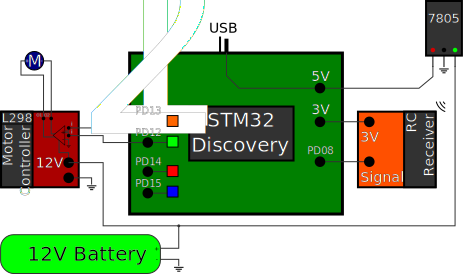
\includegraphics[width=\textwidth]{fig/circuitry}
	\caption{Kapcsolási rajz}
	\label{fig:circuitry}
\end{figure}

\section{Eredmények}

Az STM32F4-Discovery tápellátását USB kábelen, vagy az 5V Pin-en keresztül biztosíthatjuk. Ha USB-n keresztül kapja a feszültséget, a tápellátásra szolgáló Pin is +5V tápként üzemel, így biztosítva a többi +5V-os eszköz (Receiver, kormányszervó) működését. Az USB kapcsolatot megszakítva, a fő tápegységet bekapcsolva pedig a Pin árama megfordul, és már az látja el energiával a fejlesztőkártyát. Ekkor már a motor is feszültség alatt van.

A kártya felprogramozása után a működést kipróbálhatjuk még kikapcsolt állapotban, USB-s tápellátás segítségével. Mivel a szoftverben a Narancs és Zöld LED-eket vezéreljük, és az ezeknek megfelelő Pin-ek segítségével adjuk ki az arányos PWM jelet, a LED-ek segítségével in kipróbálható a várható működés, és beállítható a gáz-szervójel megfelelő semleges jelhossza. Megfelelő beállítás esetén sem a Narancssárga, sem a Zöld LED nem világít. Pozitív vagy negatív gázadásra a LED-ek a rajtuk fellépő PWM-eknek megfelelően először halványan, majd egyre fényesebben kezdenek világítani, ahogy egyre nagyobb gázt adunk. Ezzel párhuzamosan kipróbálhatjuk a kormányszervó viselkedését is.

[makro képek a led-ekről]

A kezdeti teszt után, ha helyes működést feltételezünk, végre kipróbálhatjuk a teljes rendszert. az USB kábel eltávolítása után a tápfeszültség bekapcsolásával az autó életre kel. Ha megfelelően állítottuk be a távirányító semleges gázjelét a LED-ek segítségével, az autó kezdetben nyugodt, ellenkező esetben apró lökéseket fedezhetünk fel valamelyik irányban. Miután megbizonyosodtunk a kormányszervó működéséről, óvatosan gázt adva elindulhatunk.

[kép, youtube videó link]

\section{Összefoglalás}

A dokumentáció bemutatta egy motorvezérlő modul elkészítését, mely megfelel a feladat által támasztott követelményeknek. A szoftvert sikesen fordítottuk le a beágyazott ARM Cortex M4 processzorra, a MATLAB beépített kódgeneráló funkciója segítségével, és a beágyazott eszközt egy alkalmas hardverkörnyezetben tesztelve meggyőződhettünk a helyes működésről. A kitűzott célokat sikerült megvalósítani, a rendszer a specifikációnak megfelelően működik.